\documentclass[12pt]{article}
\usepackage{indentfirst}
\usepackage{fullpage}
\usepackage{multicol,multirow}
\usepackage{tabularx}
\usepackage{ulem}
\usepackage[utf8]{inputenc}
\usepackage[russian]{babel}
\usepackage{float}
\usepackage{listings}
\usepackage{color}
\usepackage{hyperref}
\usepackage{graphicx}
\DeclareGraphicsExtensions{.png}
\graphicspath{{pics/}}
\renewcommand{\labelenumii}{\arabic{enumi}.\arabic{enumii}.}

\begin{document}
	\section*{Лабораторная работа №\,1 по курсу ИИ}
	Выполнил студент группы М8О-308Б-17 МАИ \textit{Гринин Вячеслав Витальвич}.
	
	\subsection*{Условие}
	
	Необходимо сформировать два набора данных для приложений машинного обучения. 
    
    Первый датасет должен представлять из себя табличный набор данных для задачи классификации. Второй датасет должен быть отличен от первого, и может представлять из себя набор изображений, корпус документов, другой табличный датасет или датасет из соревнования Kaggle, предназначенный для решения интересующей вас задачи машинного обучения. 
    
    Необходимо провести анализ обоих наборов данных, поставить решаемую вами задачу, определить признаки необходимые для решения задачи, в случае необходимости заняться генерацией новых признаков, устранением проблем в данных, визуализировать распределение и зависимость целевого признака от выбранных признаков. В отчете описать все проблемы, с которыми вы столкнулись и выбранные подходы к их решению.
	
	\subsection*{Метод решения}
	
	\subsubsection*{Первый датасет}
	По условию надо составить/найти такой табличный датасет, который хорошо подходит для задачи классификации. Первое что мне пришло на ум - это цвета в RGB, а точнее их яркость. Идея состоит в том, чтобы нейронная сеть по параметрам R,G,B могла определить яркость цвета. Я решил разделить цвета на тусклые и яркие. Возможно она слишком простая, но фантазии на больше мне не хватило. 
	
	Следующим делом я принялся генерировать этот самый датасет. В него будет входить 3 компонента цвета (R, G, B) и его яркость. Компоненты цвета имеют значения от 0 до 255. По сути мы получаем некоторый куб со сторонами 255x255x255, в пределах которого мы получаем различные цвета.
	
	За критерий яркости изначально хотел взять длину итогового вектора, координаты которого как раз те самые значения R, G, B. Но пришёл к выводу, что это не лучший вариант. Причиной тому послужило то, что если следовать этой идее, то серый цвет становился "ярким", хотя по факту он тусклый. Это можно было бы исправить корректировкой границ, по которым и определяется яркость, но тогда вставала другая проблема и т.д. В общем засовывать сферу в куб, надеясь на лучшее - не самая лучшая идея. В итоге решил взять вариант с чёткими границами именно по каждой координате, а не по длине итогового вектора. Таким образом я вместо сферы получаю меньшие кубы, которые находятся внутри исходного.
	
	Далее я просто сгенерировал датасет из 20000 таких значений. На этом манипуляции закончились. Анализировать тут по сути нечего, так как он можно сказать искусственный и достаточно простой. Итог получился такой: 
	
	\begin{figure}[H]
	    \centering
	    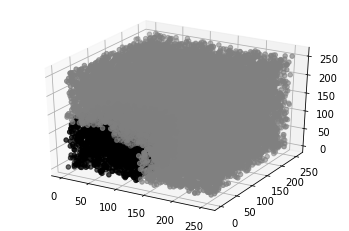
\includegraphics[scale=0.75]{Cube.png}
	    \caption{тёмные точки - тусклые цвета, светлые точки - яркие цвета}
	    \label{fig:my_label}
	\end{figure}
	
	Единственное, что стоит отметить - не равномерное распределение категорий. Цветов яркого цвета огромное количество, в то время как тусклых меньше тысячи. Объяснение этому довольно простое. Мы имеем дело с неравномерным распределением пространства, отведённого под различную яркость. Достаточно представить двумерный случай. Возьмём условно квадрат со сторонами 2x2. 
	
	\begin{figure}[H]
	    \centering
	    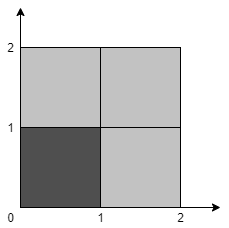
\includegraphics[scale=0.75]{distr.png}
	    \caption{тёмный квадрат - тусклые цвета, светлые квадраты - яркие цвета}
	    \label{fig:my_label}
	\end{figure}
	
	Если мы сгенерируем несколько случайных точек в пределах квадрата 2x2, то получим такую ситуацию, что большая их часть закономерно попадёт в самые светлые квадраты. Аналогичная тенденция прослеживается и для нашего трёхмерного варианта.
	
	\subsubsection*{Второй датасет}
	Так как можно взять произвольный датасет, я решил рассмотреть вариант из соревнования Kaggle, в котором содержится информация по видео роликам из сайта Youtube ({\tt https://www.kaggle.com/datasnaek/youtube-new}).
	
	Я скачал оригинальный датасет и решил избавиться от лишней информации, оставив только данные о просмотрах, лайках, дизлайках и количестве комментариев. Конечно не без проблем - ключевой проблемой были ошибки, которые связанны с кодировкой текста. Но спустя некоторое время поиска решения проблемы вопрос удалось решить.
	
	Ещё один момент связан с тем, что в отличие от искусственного датасета выше, этот датасет наверняка имеет "выбросы". Например, видео, где количество лайков ничтожно мало несмотря на большое количество просмотров. Аналогичные проблемы с комментариями - там даже все несколько хуже. 
	
	Ниже приведены иллюстрации зависимости количества лайков и комментариев от количества просмотров.
	
	\begin{figure}[h]
        \begin{minipage}[h]{0.49\linewidth}
            \center{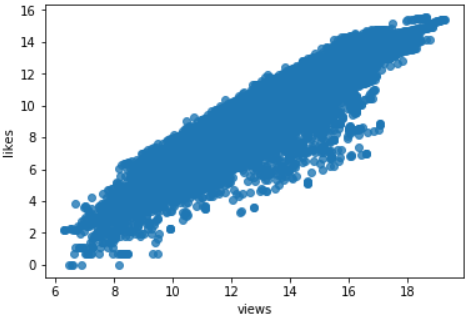
\includegraphics[width=0.95\linewidth]{likes.png} \\ а)}
        \end{minipage}
        \hfill
        \begin{minipage}[h]{0.49\linewidth}
            \center{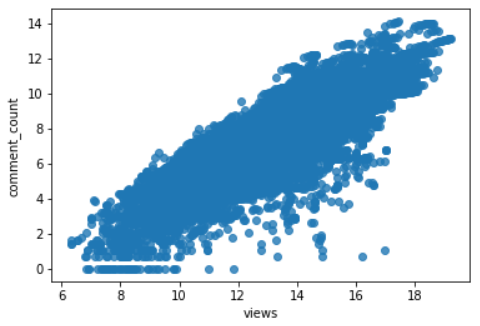
\includegraphics[width=0.95\linewidth]{comm.png} \\ б)}
        \end{minipage}
        \caption{Зависимость от количества просмотров: а) количества лайков, б) количества комментариев.}
        \label{ris:image1}
    \end{figure}
    
    В моём случае избавиться от них достаточно просто. В исходном датасете имелись столбцы, в которых стояли флаги. Флаги в свою очередь говорили о том, включены ли комментарии и лайки/дизлайки к видео. Поэтому было достаточно удалять строки, где хотя бы один из таких флагов стоял на {\tt False}.
    
	\subsection*{Выводы}
	
	Я ещё раз убедился, что у меня не получается с ходу придумать какую-либо задачу. Ту же идею с RGB я не могу назвать прям какой-то классной. Не менее странной является идея засовывания сферы в куб. Конечно изначально и так было понятно, что это ни к чему хорошему не приведёт, но попробовать же хочется...
	
	Если отбросить мысли выше, то эта лабораторная дала понять, что перед составлением датасета лучше формализовать задачу, которую надо решить. Помимо этого появилось некоторое представление о том, каким образом отбираются те или иные признаки. Банально нужно понимать, как те или иные признаки зависят друг от друга и зависят ли вообще.
	
\end{document}